\documentclass[11pt]{article}
\usepackage[a4paper, portrait, margin=1in]{geometry}
\usepackage{multirow}
\usepackage{booktabs}
\usepackage{adjustbox}
\usepackage{hyperref}
\usepackage{listings}
\usepackage{fancyvrb}
\usepackage{moreverb}
\usepackage{xcolor}
\usepackage{listings}
\usepackage{tcolorbox}
\usepackage{color, colortbl}
\usepackage{float}

\definecolor{swotW}{RGB}{247,193,139}
\definecolor{swotO}{RGB}{173,208,187}
\definecolor{swotT}{RGB}{192,165,184}
%\definecolor{myblue}{rgb}{0.54, 0.81, 0.94}
\definecolor{myblue}{rgb}{0.63, 0.79, 0.95}
\definecolor{mypink}{rgb}{1.0, 0.99, 1.0}

\geometry{a4paper}

\begin{document}
\pagestyle{plain}


\title{Advanced Systems Lab -- First Milestone}

\author{Name: \emph{Rabeeh Karimi Mahabadi}\\Legi number: \emph{13923941}}

\maketitle

\newpage

\tableofcontents
\newpage


\section{System Description}\label{sec:system-description}

\subsection{Database}\label{sec:database}
The database underlying the project is \emph{Postgresql}, and the version used 
in this project is \emph{Postgresql 9.3}.

\subsubsection{Schema and Indexes}\label{sec:schema-and-indexes}
I used two tables for storing the messages and queues. In which \emph{queue\_id} in message
table references the \emph{id} in queue table to prevent invalid \emph{queue\_ids} to be inserted into the 
message table. Additionally, it would be a good idea to consider the third table for user authentications. However, I 
did not consider the user table as it was not directly asked in the project 
specification. The Database schemas are shown below:

\begin{table}[!ht]
\centering
\begin{tabular}{lll}
\toprule
Field & Type & Description \\ \midrule
\emph{id} & Serial & Primary key \\
\emph{creation\_time} & Timestamp & Time of the queue creation \\
\emph{creator\_id} & Integer & Not null, id of the creator of the queue  \\\bottomrule
\end{tabular}
\caption{Queue table}
\end{table}

\begin{table}[!ht]
\centering
\begin{tabular}{lll}
\toprule
Field & Type & Description \\ \midrule
\emph{id}            & Serial    & Primary key \\
\emph{sender\_id}    & Integer   & Not null, id of the sender \\
\emph{receiver\_id}  & Integer   & Id of the receiver          \\
\emph{queue\_id}     & Integer   & Not null, id of the queue, references \emph{id} in queue table  \\
\emph{arrival\_time} & Timestamp & Time of arrival of the message   \\
\emph{message}       & Text      & Message, not null  \\\bottomrule
\end{tabular}
\caption{Message table}
\end{table}

In order to speed up the queries, I looked at all the possible queries of the 
system, and used indexes for the ones which need \emph{ORDER BY} operation. 
The reasoning is that, if one does not use indexes for these type of queries, 
for getting the only topmost message, all the messages should be read from
disk and get sorted which will become very costly, specially if the query is 
executed several times in a short period of time. Furthermore, for this project
in which the system needs to insert several messages per second to the database,
the size of database will grow over time, and without indexes the queries would take 
much more time as it needs to sort huge amount of data. I considered the following three indexes for the project:
\begin{itemize}
\item {\emph{queue\_id}, \emph{arrival\_time}}
\item {\emph{receiver\_id}, \emph{queue\_id}}
\item {\emph{sender\_id}, \emph{arrival\_time}}
\end{itemize}

The first index is useful for reading the topmost message from the queue, the 
query is shown below:

\begin{center}
\begin{tcolorbox}[width=\textwidth,title={Query topmost message in a queue for a 
particular receiver},outer arc=0mm]    
\begin{verbatim}
    SELECT id, sender_id, message FROM message
    WHERE queue_id = _queue_id AND 
    (receiver_id IS NULL OR receiver_id = _receiver_id)
    ORDER BY queue_id, arrival_time 
    LIMIT 1;  
\end{verbatim}
\end{tcolorbox}  
\end{center}

The second index is very useful to improving the performance 
in querying the queues as shown below, this query can be done without 
\emph{ORDER BY}, but by using \emph{ORDER BY} the query planer would understand to 
make a use of the indexes:

\begin{center}
\begin{tcolorbox}[width=\textwidth, title={Query queues},outer arc=0mm]    
\begin{verbatim}
SELECT DISTINCT queue_id FROM message
WHERE receiver_id=_receiver_id
ORDER BY queue_id;
\end{verbatim}
\end{tcolorbox}  
\end{center}

The third index is used to speed up querying the message of a particular 
sender:

\begin{center}
\begin{tcolorbox}[width=\textwidth,title={Query message of a particular sender},outer arc=0mm]    
\begin{verbatim}
SELECT  id, sender_id, message FROM message
WHERE  _sender_id = sender_id AND
(receiver_id IS NULL OR receiver_id = _receiver_id)
ORDER BY sender_id, arrival_time
\end{verbatim}
\end{tcolorbox}  
\end{center}

\subsubsection{Stored Procedures}\label{sec:stored-procedures}
I used stored procedure for all the queries that systems need to do, also to create
tables, indexes, and delete them. The benefit of stored procedure is that they increase 
the performance of the database because:
\begin{itemize}
 \item it reduces the amount of information sent to the database server. It becomes more 
 important when the bandwidth of the network is less. 
 \item compilation step is required once when the stored procedure is created, and it 
 does not require recompilation before each time execution.
 \item it helps in reusability of the SQL code. 
\end{itemize}


\subsubsection{Design decisions}\label{sec:design-decisions}
I translated send message to \emph{INSERT}, and peek and query the messages
to \emph{SELECT} in SQL. For the popping of the messages, in order to avoid race
condition, I used \emph{SELECT ... FOR UPDATE} statement, to lock only one 
row of the table when executing the pop statement. It helps to improve the performance
of the database as the number of records locked at any given time for pop 
operation are kept to the minimum.

I tried to tweak a little bit the parameters in the database configuration file, and I set 
\emph{shared\_buffer} to 3GB, \emph{work\_mem} to 4MB, also I increased 
the number of the \emph{checkpoint\_segments} to 32 as initially I got the 
error message that ``checkpoints are occurring too frequently'' during my 
experiments, so I increased the number of \emph{checkpoint\_segments} to keep
the number of checkpoint operations happening during the experiments as small as 
possible. I also enabled asynchronous commit which is an option that allows 
transactions to complete more quickly. In general, I tried to increase the 
memory limits to allow having more throughput for the experiment. However, these values 
are far from the optimal values. By careful selection of the parameters, one could
be able to get a better results.

\subsubsection{Performance characteristics}\label{sec:performance-characteristics}
Inorder to evaluate the performance of the database, I measured throughput and 
response time over different number of database connections for three different experiments:
\begin{itemize}
 \item Only read operation
 \item Only write operation
 \item Combination of read (50 \%), write (25 \%), send (25 \%) operations: Percantage of different
 workloads have been chosen in a way to keep the database size constant over time.
\end{itemize}

I ran all the experiments for 3 minutes. Throughput values are averaged for the 
whole duration of the experiment. Response time values are averaged for every
20 seconds and I computed the average of the all intervals. In all the experiments, 
I sent as many requests as possible with \emph{think\_time} of zero.
Also, \emph{15000} messages are initially
distributed over \emph{20} queues in database. I used \emph{m3.large} instance for the database 
machine. The logs can be found in \emph{logs/database}. Response times and throughputs
are shown in figures \ref{fig:db_response_time}, \ref{fig:db_thoughput}. As expected,
\emph{Read} experiment has the most throughput, and the throughput of \emph{Write} 
experiment is less than that. The reasoning is that in the write operation, data is flushed 
to the disk which is time consuming. \emph{Combination} experiment throughput 
is bigger than write operation, because it has peek operations which are not expensive
Also, one should consider that during the \emph{write}, and \emph{delete} operations
database needs to update also the indexes, which also plays a role in decreasing the 
throughput for \emph{write}, and \emph{combination} experiments. 

Furthermore, I can see that I have the best performance for \emph{16} database connections.
Increading the database connections up to \emph{16} connections, make a substantial
improvement in throughput. However, after \emph{16} connections, adding more connections
does not affect the throughput that much and even in some cases decreases it. The behavior
can be explained by the fact that the machine I used for database has only two cores, and 
by adding more database connections, processes needs to fight for avialable resources
which decreases the performance. However, in \emph{16-24} connections, because the 
time when processes are blocked for reading or writing from file system,
can be used to answer more requests, the throughput has been increased.
In addition, response time also increases substantially by adding more database 
connections.The reasoning, can again be attributed to the fact that processes needs to 
fight for the resources with having more database connections. 

\begin{figure}[!ht]
  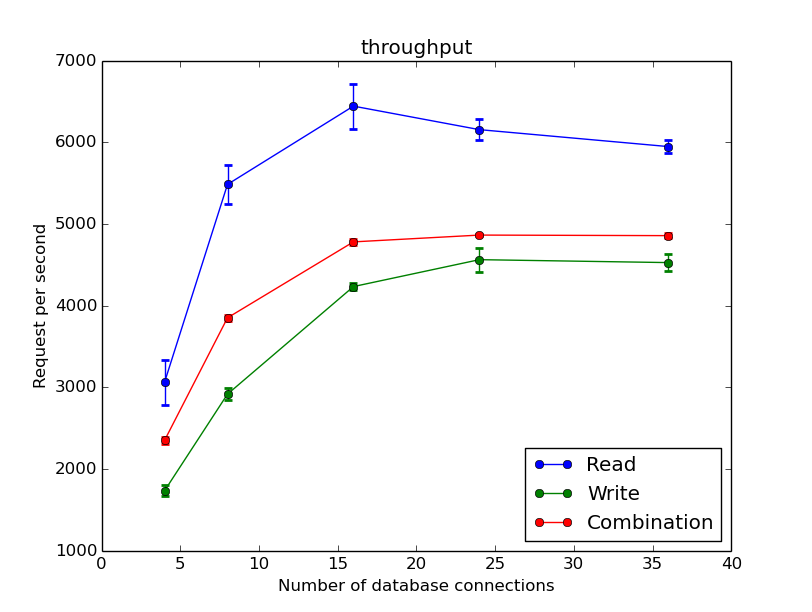
\includegraphics[height=0.4\textheight,page=1]{figures/db_throughput}
  \centering
  \caption{Database throughput over different number of database connections
  for three different workloads}
  \label{fig:db_thoughput}
\end{figure}

\begin{figure}[!ht]
  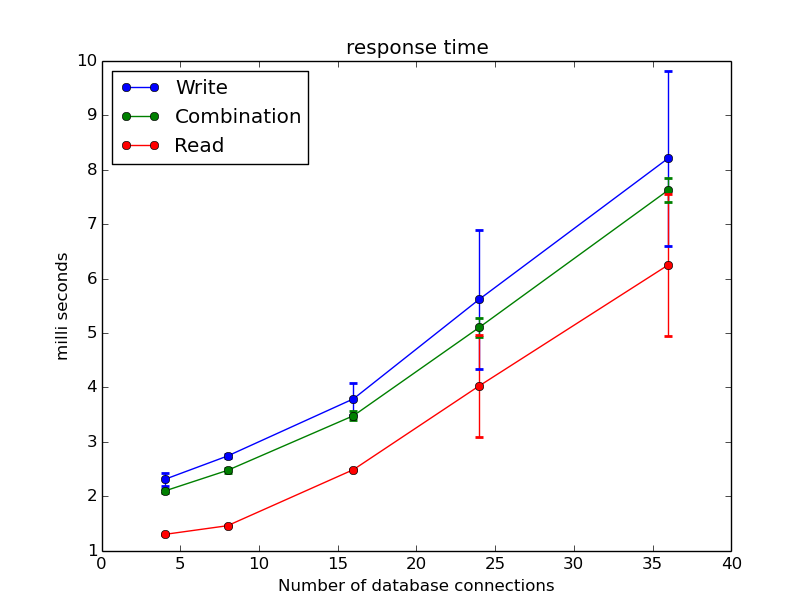
\includegraphics[height=0.4\textheight,page=1]{figures/db_response_time}
  \centering
  \caption{Database response time over different number of database connections
  for three different workloads}
  \label{fig:db_response_time}
\end{figure}

\subsection{Middleware}\label{sec:middleware}

\subsubsection{Design overview}\label{sec:design-overview}

The system overall design is depicted in figure \ref{fig:system}. The input data is read
and buffered asynchronously by \emph{connectionManager}. \emph{ConnectionManager}, creates a 
\emph{requestDispatcher} object for each incoming request. The job is added to the frontend pool,
where a worker from the frontend pool executes the task. During which,\emph{requestDispatcher}
creates the corresponding backend task and add it to the backend pool. A worker from backend pool
takes the task and executes it to the database. After that, a \emph{responseDispatcher} is 
created for the received response, and the task is added to the Frontend pool. 
Finally, A worker from frontend pool executes the task and delivers the response to the client. 

\begin{figure}[!ht]
  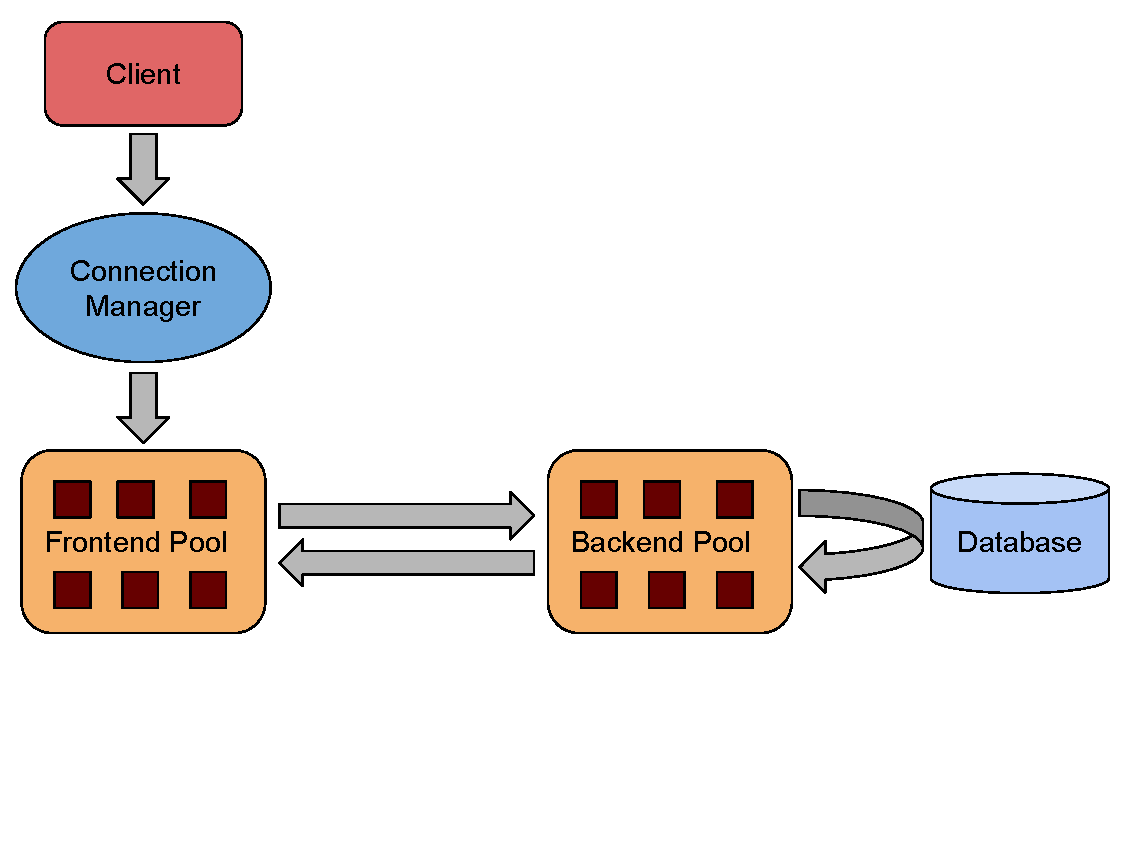
\includegraphics[height=0.35\textheight,page=1]{figures/system}
  \centering
  \caption{System overall design}
  \label{fig:system}
\end{figure}

A few points should be mentioned about the design: 
\begin{itemize}
 \item Inorder to avoid networking overhead, each clients opens the connection once 
 and use this connection to send all of its requests.
 \item To use resources as efficiently as possible, \emph{Java nio} package is used 
 to handle incoming requests and build a highly scalable system. Hence, I did not used the intuitive approach of 
 \emph{thread-per-connection}. 
 \item Two different backend and fronend tasks are considered in the system, and 
 the goal was to keep the backend tasks as light as possible. Backend tasks are 
 used to execute the query to the database, and frontend tasks are used to deliver 
 the message to the client back, and also to parse a request from the client.
\end{itemize}

\subsubsection{Interfacing with clients}\label{sec:interfacing-with-clients}
Clients use blocking I/O, and the middleware uses non-blocking I/O to handle the 
requests. I also considered the following serialization scheme:

\begin{figure}[!ht]
  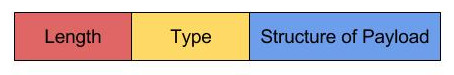
\includegraphics[width=0.64\textwidth,page=1]{figures/serialization}
  \centering
  \caption{Serialization scheme}
  \label{fig:serialization}
\end{figure}

So each request starts with 4 bytes length of the payload, then type of the request,
and then the actual payload. Different requests have different structure depending 
on their type. To improve the transmission speed \emph{DataOutputStream} and 
\emph{DataInputStream} are used because these methods can read and write an integer, 
a double and a line as a whole at a time instead of byte by byte.

\subsubsection{Queuing and Connection pool to database}\label{sec:queuing-and-connection-pool-to-database}
Before creating the backend pool, one database connection is assigned to each thread.
The connection is created once, and is used to execute all queries to the database.
The queuing mechanism used in the project is done by \emph{java ThreadPoolExecutor} 
which construct a threadPool and uses \emph{LinkedBlockingQueue} for queuing the tasks.
Making connections once and assigning them to each thread, while avoiding creating
connections each time, improves the performance substantially.

\subsubsection{Performance characteristics}\label{sec:performance-characteristics-1}
For testing the middleware scalability, I introduced a new request type called \emph{Echo}
in which a client sends a \emph{string} to the middleware, and middleware sends the 
same message back. This way, the request is isolated from the database, and one could 
test the performance of the middleware separately. In this experiment, I used different 
number of clients, and a fixed number of \emph{30 frontendpool workers}, and 
one middleware instance. Clients send as much request as possible with \emph{think\_time}
of zero, and I measured throughput and response\-time for each set\-up the same way I did in database experiment\ref{sec:performance-characteristics}.
I used \emph{t2.medium} instance both for client and middleware. 
Throughput and response\-times are shown in figures \ref{fig:middleware-throughput} and \ref{fig:middleware-response-time}.
As it is depicted in the figures, one middleware instance can support 64 clients sending 
\emph{185000} requests per second. Also, the reponse time for 
\emph{64} clients is around twice of the response time for 
\emph{32} clients, and still within a very reasonable time.
In summary, using \emph{non-blocking I/O} clearly made a very 
scalable architecture for handling several requests per second. 
The \emph{logs} for this experiments can be found in \emph{logs/middleware\_clients}
folder.

\begin{figure}[H]
  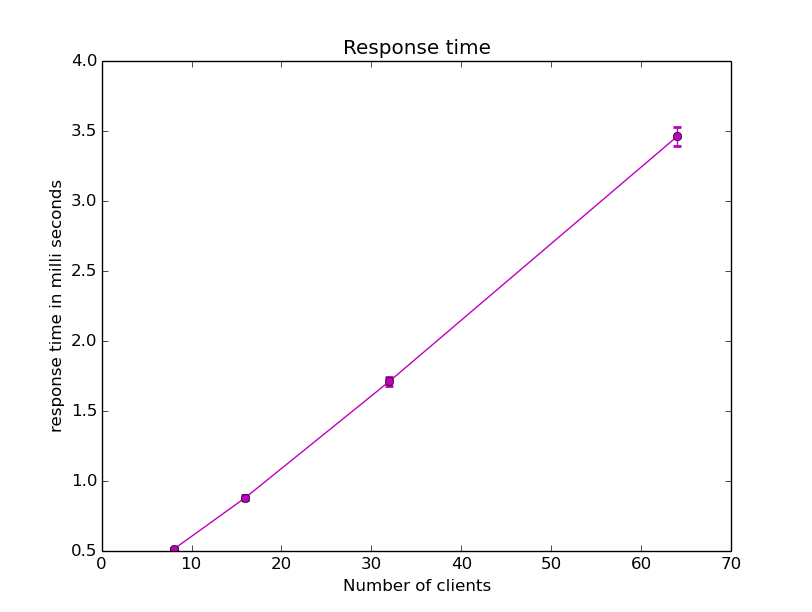
\includegraphics[width=0.7\textwidth,page=1]{figures/middleware-response-time}
  \centering
  \caption{Response-time with one middleware and different number of clients}
  \label{fig:middleware-response-time}
\end{figure}


\begin{figure}[H]
  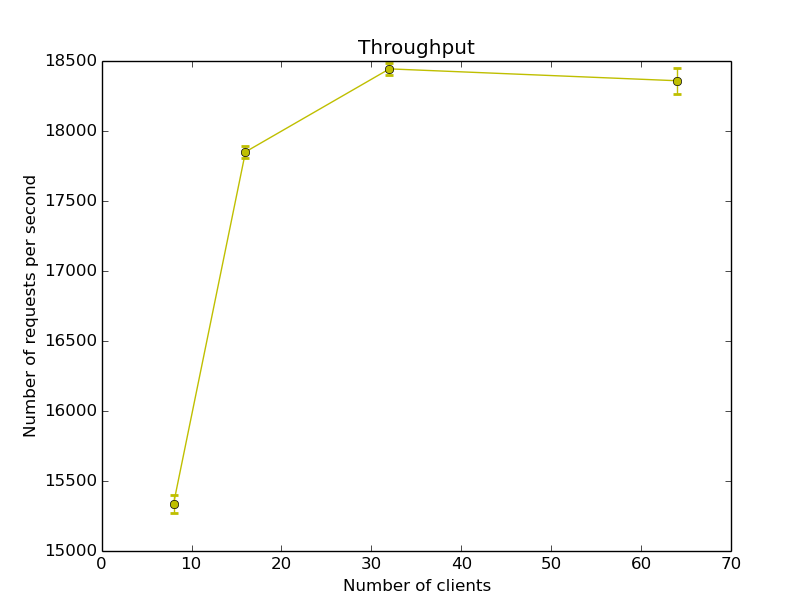
\includegraphics[width=0.7\textwidth,page=1]{figures/middleware-throughput}
  \centering
  \caption{Throughput with one middleware and different number of clients}
  \label{fig:middleware-throughput}
\end{figure}


\subsection{Clients}\label{sec:clients}

\subsubsection{Design and interface}\label{sec:design-and-interface}
Clients use non-blocking I/O. I implemented two main strategies for generating loads
for the experiments:
\begin{itemize}
 \item Sending as many request as possible with a parameter \emph{think\_time}
 that could be set for each experiment \footnote{\emph{FlowRequestRunner}}
 \item Sending the request in a regular intervals for instance sending requests
 every \emph{1ms}\footnote{\emph{RegularRateRunner}}
\end{itemize}
Each client has assigned a \emph{log file} in which it writes its response time values
Also, I considered printing ``\emph{One Block}`` after every second in log files,
such that I can divide the response times in one second intervals and use them in 
my computations when I need to average the response times over a specific intervals.


\subsubsection{Instrumentation}\label{sec:instrumentation}

\subsubsection{Workloads and deployment}\label{sec:workloads-and-deployment}
Each client can send one type of the request: query, peek, pop, and send. In order to 
generate the workload of different combinations for instance query and pop, one 
could use different clients for this purpose, and assign one operation to 
each client. Number of clients and their corresponding
operations can be set by the argument to the program. All possible parameters of the 
program such as number of users, length of the message, etc can be set in the code
\footnote{\emph{Parameters}}. I considered generating random string of 
specific length for the message the client wants to send. I also considered generating
the \emph{queue\_id} and \emph{receiver\_id} randomly to simulate more realistic 
workload generation.

\subsubsection{Sanity checks}\label{sec:sanity-checks}
For ensuring correct load generation and validity of responses, each client will check
if it has received a valid response, and throws an exception otherwise in the log file.
Then, one could check all the log files and repeat the experiments in case of 
any error occurance during the experiment.

\section{Experimental Setup}\label{sec:experimental-setup}

For database I used \emph{m3.large} because it has \emph{7.5 GB} of memory, and the 
memory was large enough to be suitable for my experiments. 
For server and clients, I used \emph{t2.medium} instance, because I do not need that 
much memory on client and server, but I need more CPU, and this instance has \emph{2}
\emph{CPU} and \emph{3.75} GB memory. 

\subsection{System Configurations}\label{sec:system-configurations}
In general, the system consists of one database, a few number of middlewares 
and several clients which are connected to the middleware instances. Clients send the requests 
to the middleware, middleware parse the request and send the task to the database,
when the results are prepared, middleware send back the response to the clients. 


\subsection{Configuration and Deployment mechanisms}\label{sec:configuration-and-deployment-mechanisms}
Inorder to run the experiments, I wrote a \emph{bash} script for each experiment, 
the scripts are in the folder of \emph{bash\_scripts}. All the parameters that one need to set
to run the experiments such as \emph{server inet address}, \emph{message length}, etc 
are passed as arguments to the \emph{jar files} in the scripts. 
I used up to 2 middleware instances in my experiments.
During development of the system, I wrote several \emph{Junit} tests to make sure 
about the functionality of the each part of the system.

For computing different statistics from the results of the experiments such as 
computing the \emph{throughput} and \emph{response\_time}, I wrote 
two \emph{python} scripts which are in the folder of \emph{analyze}.
The first one is called \emph{analyze\_measurements.py}
for computing the mean and standard deviation for throughput and response-time of 
each experiment. The second script is called \emph{generate\_time\_series.py}. This 
script is only used for the \emph{stability} experiment for generation
the response time and throughput values for the longer runs.

\section{Evaluation}\label{sec:evaluation}

\subsection{System Stability}\label{sec:system-stability}
For this experiment, I considered 40 clients which are sending 25 requests 
per second and I distribute their requests into two middleware instances. 
So, in total system receive the load of 1000 requests per second. 20 clients 
send the request to the first middleware instance and 20 other clients send their 
requests to the second middleware instance.
I used \emph{m3.large} instance
for the database, and two \emph{t2.medium} instances for two middlewares, 
and another \emph{t2.medium} instance for the clients. I initialize the database 
with \emph{2000} messages. Number of backend pool workers is set to \emph{10} so having 
two middleware instances, in total 20 database connections are used. I set this number 
because in the database experiments, I observed that system achieve the maximum performance for 
around 15-24 database connections. Number of FrontendPool workers does not really 
matter, as shown in the middleware experiments, database is the bottleneck and 
with 15 frontend workers middleware should be able to handle a large number of 
requests. I used a workload with combination
of pop and send with equal portion of each operation such that the size of the database remains the same over time.
The parameters I used for this experiments 
are shown in table \ref{table:stability}. The trace of system throughput and response time is depicted in figures 
\ref{fig:stability_throughput}, and \ref{fig:stability_response_time}.

\begin{table}[ht]
\centering
\begin{tabular}{c|ccccccc}
\hline
\rowcolor{myblue}
Message Length        & 200 \\
\rowcolor{mypink}
Number of clients     & 40 \\
\rowcolor{myblue}
Number of middlewares & 2 \\
\rowcolor{mypink}
Experiment time       & 30 minutes \\
\rowcolor{myblue}
Frontend pool size    & 15 \\
\rowcolor{mypink}
Database pool size    & 10 \\
\rowcolor{myblue}
Rate of requests      & 25 requests per second \\ 
\rowcolor{mypink}
Workload              & Combination of pop, and write (50 \% each) \\
\hline
\end{tabular}
\centering
\caption{Configuration used in the stability experiment}
\label{table:stability}
\end{table}

\begin{figure}[H]
  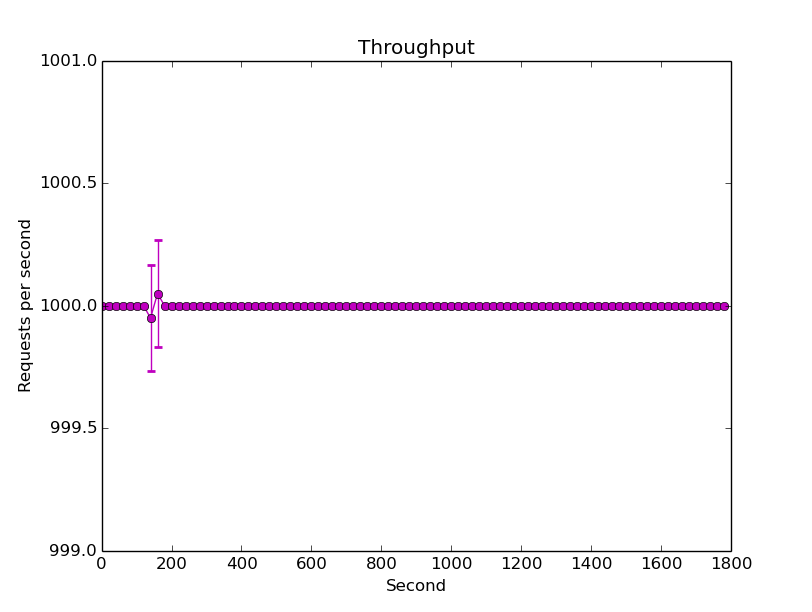
\includegraphics[width=0.6\textwidth,page=1]{figures/stability_throughput}
  \centering
  \caption{Throughput of the system over 30 minutes run for 1000 requests per second}
  \label{fig:stability_throughput}
\end{figure}

\begin{figure}[H]
  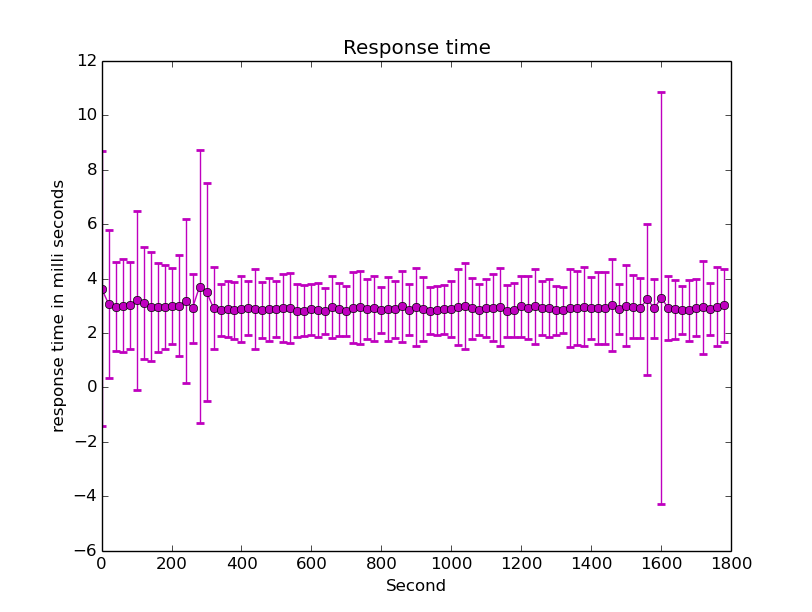
\includegraphics[width=0.6\textwidth,page=1]{figures/stability_response_time}
  \centering
  \caption{Response time of the system over 30 minutes run for 1000 requests per second}
  \label{fig:stability_response_time}
\end{figure}

For sanity check, each client, checks the response it receives, and 
if the response is invalid it logs an error in the log files. 
The logs for this experiment can be found in the folder \emph{logs/stability}.
Response time and throughput values are averaged over \emph{20} seconds intervals.
The response times and throughput values are quite stable. Small variances in the 
response times can be attributed to the shared nature of \emph{AWS EC2} environment.

In the second part of this experiment, I applied 4 times more load, 100 request per second,
with the same configuration as the first experiment. In total, the load on the 
system will be 4000 request per second. I chose these values because in the experiment
shown in section \ref{sec:performance-characteristics}, the system is able to 
support up to 4000 write operations per second and pop and write operations have roughly 
the same throughput and response times, so the system should be able to
handle 4000 requests per second. The logs for this experiment can be found in 
\emph{logs/stability\-2}, and the results are depicted in figures \ref{fig:stability-2-response-time}
and \ref{fig:stability-2-throughput}. The results show that the throughput and 
response times remains stable. The response time and throughput values are 
averaged over 20 seconds intervals. As we can see, every drop in the 
throughput graph is followed by a spark, meaning that the requests in the 
system are not lost, but it indicates that a request is started in the 
previous interval but completed in the next interval. The variances in the 
response times are about \emph{6ms}, which is quite small and can be attributed 
to the shared nature of \emph{AWS EC2} environment.

\begin{figure}[H]
  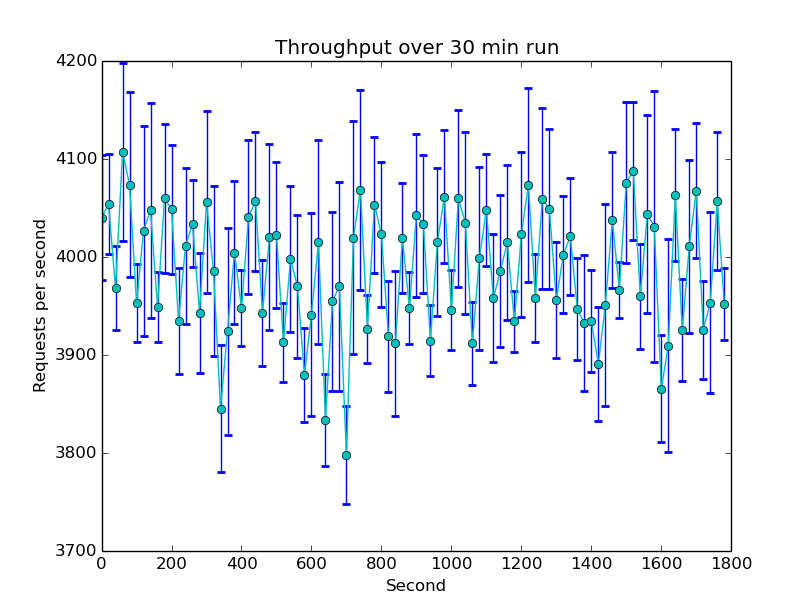
\includegraphics[width=0.7\textwidth,page=1]{figures/stability_throughput_2}
  \centering
  \caption{Throughput of the system over 30 minutes run for 4000 requests per second}
  \label{fig:stability-2-throughput}
\end{figure}

\begin{figure}[H]
  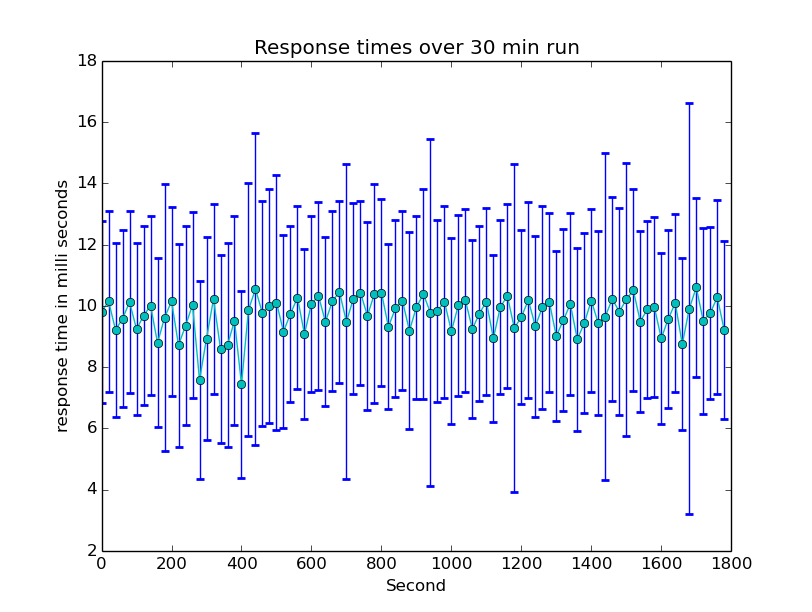
\includegraphics[width=0.7\textwidth,page=1]{figures/stability_response_time_2}
  \centering
  \caption{Response time of the system over 30 minutes run for 4000 requests per second}
  \label{fig:stability-2-response-time}
\end{figure}


\subsection{$2^k$ Experiment}\label{sec:k-experiment}
In this experiment, I would like to analyze different possible factors on 
system throughput. I considered the factors in table \ref{table:factor_throughput_2k}.
Values have been chosen in a way that throughput for Level 1 is expected to be higher than the throughput for level -1.
For instance, having 2 middleware instance and smaller message sizes will help to 
have more throughput. Throughputs values are averaged between three times repetition of the 
experiments each one for 5 minutes duration, statistics and logs can be found in \emph{logs/factorial}.

\begin{table}[ht]
\centering
\begin{tabular}{l*{3}{c}r}
Factor                   & Level -1 & Level 1  \\
\hline
A: Message Length           & 1200 & 200   \\
B: Number of middlewares    & 1    & 2  \\
C: Number of clients        & 32 & 64  \\
\end{tabular}
\label{table:factor_throughput_2k}
\caption{Factors for $2^k$ throughput experiment}
\end{table}

The results of the $2^k$ throughput experiment have been shown in 
\ref{table:2k_throughput}. Based on the results, number of clients have the 
most substantial affect on throughput. The reasoning is that, as it was 
shown in middleware experiment, one middleware instance can easily handle upto 18500 requests per second
and middleware design is highly scalable, so having more middleware instances 
does not help to have more throughput as only one middleware instance is already enough.
Furthermore, message length only has a negligible affect on throughput as 
network transmission time constitutes only small fraction of the final response time
values.

\begin{table}[!ht]
\begin{adjustbox}{width=1\textwidth}
\begin{tabular}{*{12}r}  \toprule
\emph{I}  &  \emph{A} & \emph{B}  & \emph{C} & \emph{AB} & \emph{AC} & \emph{BC} & \emph{ABC} & \emph{TP}  \\\midrule
1  & -1 & -1 & -1 &  1  &  1  &  1  & -1  &  3909.3 \\
1  &  1 & -1 & -1 & -1  & -1  &  1  &  1  &  4040.9 \\
1  & -1 &  1 & -1 & -1  &  1  & -1  &  1  &  4851.8 \\
1  &  1 &  1 & -1 &  1  & -1  & -1  & -1  &  4784.0 \\ 
1  & -1 & -1 &  1 &  1  & -1  & -1  &  1  &  3896.6 \\
1  &  1 & -1 &  1 & -1  &  1  & -1  & -1  &  3966.2 \\
1  & -1 &  1 &  1 & -1  & -1  &  1  & -1  &  2174.6 \\
1  &  1 &  1 &  1 &  1  &  1  &  1  &  1  &  2301.5 \\\hline
 29925 &  260.30 & -1701.1 & -5247.1 & -142.10 &  132.70 &-5072.3 &  256.70 & ToTal\\
 3740.625 &32.538 &  -212.637 &  -655.888 &   -17.762  &   16.587 &  -634.038& 32.087 & ToTal/8 \\
 Variation & 0.120294 \% &   5.137535 \% &  48.880291 \% &    0.035850\% &   0.031263 \% &   45.677778 \% & 0.116989 \%  \\
 \hline
\end{tabular}
\end{adjustbox}
 \caption{Sign table for throughput}
 \label{table:2k_throughput}
\centering
\end{table}

In the second part of this experiment, I tried to analyze the same factors affect
on response time. Factors chosen for this experiment are shown in table
\ref{table:f_2k_response_time}. Again, factors have been chosen in a way that 
response time for Level -1 is expected to be smaller than response time for 
factors in Level 1 because by having larger message length and smaller middleware insatnce 
response time is expected to increase as for larger message sizes, it is expected to 
have more networking overhead. In additon, having less clients means less load 
for the system and hence shorter response times. The experiment is ran for 
5 minutes, and response time values are averaged every 20 seconds.
The results of the experiment are shown in table \ref{table:response_2k}.
Based on the results, again one can see that number of clients have the 
biggest affect on response time. The same reasoning as the throughput experiment
also applies here. Also, number of middleware nodes have a very small affect 
which is meaningful as increasing the number of middleware nodes could 
decrease the latency for a small amount. 

\begin{table}[ht]
\centering
\begin{tabular}{l*{3}{c}r}
Factor                   & Level -1 & Level 1  \\
\hline
A: Message Length           & 200 & 1200   \\
B: Number of middlewares    & 2    & 1  \\
C: Number of clients        & 32 & 64  \\
\end{tabular}
\caption{Factors for $2^k$ response time experiment}
\label{table:f_2k_response_time}
\end{table}

\begin{table}[!ht]
\begin{adjustbox}{width=1\textwidth}
\begin{tabular}{*{12}r}  \toprule
\emph{I} &  \emph{A} & \emph{B}  & \emph{C} & \emph{AB} & \emph{AC} & \emph{BC} & \emph{ABC} & \emph{RT}  \\\midrule
1  & -1 & -1 & -1 &  1  &  1  &  1  & -1  &  6.9675 \\
1  &  1 & -1 & -1 & -1  & -1  &  1  &  1  &  6.7175 \\
1  & -1 &  1 & -1 & -1  &  1  & -1  &  1  &  7.8725\\
1  &  1 &  1 & -1 &  1  & -1  & -1  & -1  &  8.2642 \\ 
1  & -1 & -1 &  1 &  1  & -1  & -1  &  1  &  29.858 \\
1  &  1 & -1 &  1 & -1  &  1  & -1  & -1  &  31.567 \\
1  & -1 &  1 &  1 & -1  & -1  &  1  & -1  &  16.161 \\
1  &  1 &  1 &  1 &  1  &  1  &  1  &  1  &  16.461 \\\hline
124.1654 & 2.2556 &  -26.4396 &   63.9286 &   -1.0806 &    1.7624 &  -31.1664 & -1.7374 & ToTal\\
15.52068 & 0.28195 &  -3.30495&    7.99107&   -0.13508&    0.22030&   -3.89580& -0.21717 & Total/8 \\
Variation & 0.088181 \% &   12.116054 \% &  70.833924 \% &    0.020240\% &   0.053834\%  &  16.835450\% & 0.052316\%  \\ \hline    
\end{tabular}
\end{adjustbox}
\caption{Sign table for response time}
\label{table:response_2k}
\centering
\end{table}


\subsection{System Throughput}\label{sec:system-throughput}

In order to measure the maximum throughput of the system, 
I used all the information I learned from my system in previous experiments.
In section \ref{sec:performance-characteristics}, I observed that the system
can achieve the best throughput for \emph{16-24} database connections. In addition,
based on the experiment in section \ref{sec:performance-characteristics-1},
one middleware instance can easily support up to 18000 requests per second. 
Furthermore, in section \ref{sec:k-experiment}, I observed that number of 
clients has the most prominent affect on throughput. Hence, for this experiment
I came up with the following set up. I will use 16 database connection, 30 Fronend
Pool workers, and a workload of combination of the all of the system operations
meanning that I considered \emph{pop}, \emph{peek}, \emph{send}, \emph{query}
each one with equal portion, then I measured  
throughput and response time for different number of clients. I considered \emph{think\_time} of zero 
for this experiment. Throughput and response times are shown in figures \ref{fig:th-th}
and \ref{fig:th-rs}.


\begin{figure}[H]
  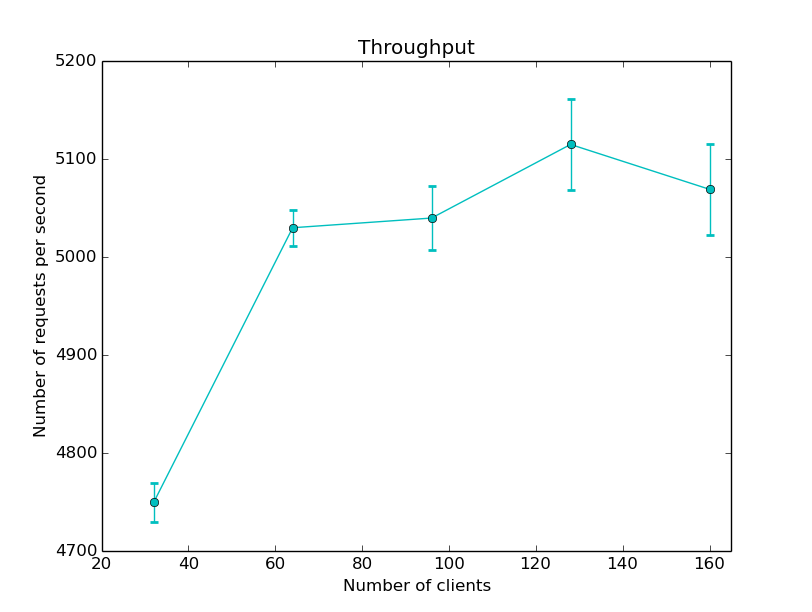
\includegraphics[width=0.7\textwidth,page=1]{figures/max_throughput_throughput}
  \centering
  \caption{Throughput of the system for different number of clients}
  \label{fig:th-th}
\end{figure}

\begin{figure}[H]
  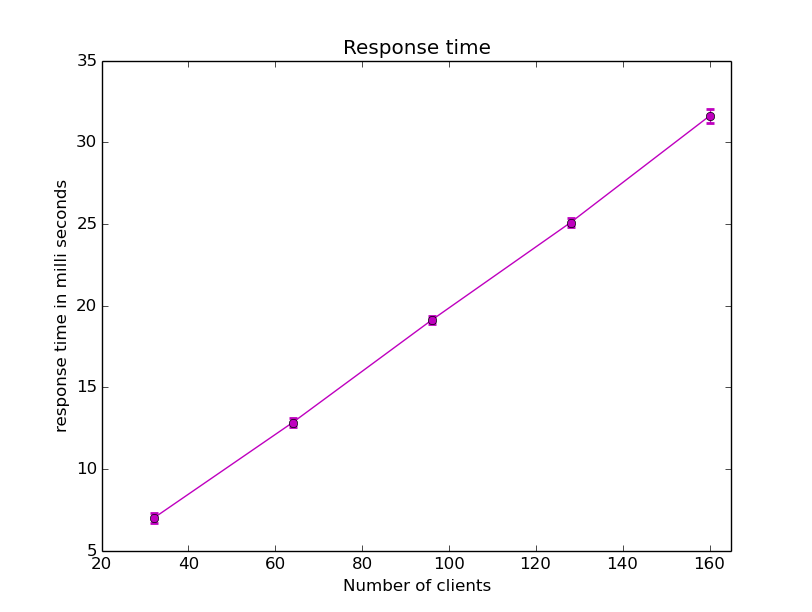
\includegraphics[width=0.7\textwidth,page=1]{figures/max_throughput_response_time}
  \centering
  \caption{Response time of the system for different number of clients}
  \label{fig:th-rs}
\end{figure}

As expected the max throughput is around 5000 requests per seconds which is around the max throughput of the 
database. This experiment shows that database is the bottleneck in this design. 
Also, we should consider that we have \emph{Query} operations in this experiment
which is not considered in the database experiment, however, it should be 
roughly of the same cost as \emph{Peek} operation. In addition, in this experiment
I considered 16 database connections for each middleware instance which also 
helps to have optimal throuhput.


\subsection{System Scalability}\label{sec:system-scalability}
In this section, I would like to explore the scalability of the system based on the 
results obtained in the previous experiments. In section \ref{sec:performance-characteristics}
, we observed that 12 to 24 database connections can achieve maximum performance.
Furthermore, in section \ref{sec:system-throughput}, it was shown that above 80
clients should be able to create enough load to saturate the database.
For this experiment, I choose combination of the \emph{peek}, \emph{pop},
\emph{query}, \emph{send} operations, each one with \emph{25\%} contribution to the 
whole load to simulate the realistic load on the system. I chose 96 clients, because first, based on the
experiment in \ref{sec:performance-characteristics} they can generate enough load to 
saturate the database, second, this number is divisable by 4, 8, and 12 which
I need in this experiment to distribute the number of clients equally 
between middlewares nodes and 4 different operations.
To sum up, I run this experiment for 96 clients, and different number of middlewares 
\emph{1,2,3}, and each middleware has either 6 or 10 database connections. 
The logs for this experiment can be found in folder \emph{logs/scalability}.
Obtained throughput and response times are shown in \ref{fig:scalability_throughput}, and 
\ref{fig:scalability_response_time}. The results show that 
up to 20 database connections are enough to have the 
maximum performance. This is consistent with the experiments 
conducted in \ref{sec:performance-characteristics}, in which 
we observed that 15-24 database connections will result in maximum 
performance. The second point from the figure \ref{fig:scalability_throughput}
is that throughput for the configuration of 3 middleware instance with 
6 or 10 database connections per middleware are roughly the same. This means that 
with 30 database connections(10 database connection per instance),
the system cannot saturate all of them. However, in the first configuration
with 3 middleware instance and 18 database connections, database
connections are saturated and the system uses all of them optimally.
By looking at the response time graph, we observe that with 6-10
database connections in one middleware instance, response time values 
are very high, meaning that the system has too few database connections 
to handle the requests. Adding more database connections improve the 
reponse times, and one could have the optimal performance for 
12-20 database connections. Furthermore, I should mention that 
number of middleware instances does not really affect the throughput 
or response times. As shown in section \ref{sec:performance-characteristics-1}
one middleware instance can handle much more requests than database, and database 
is the bottleneck in this design.

\begin{figure}[ht]
  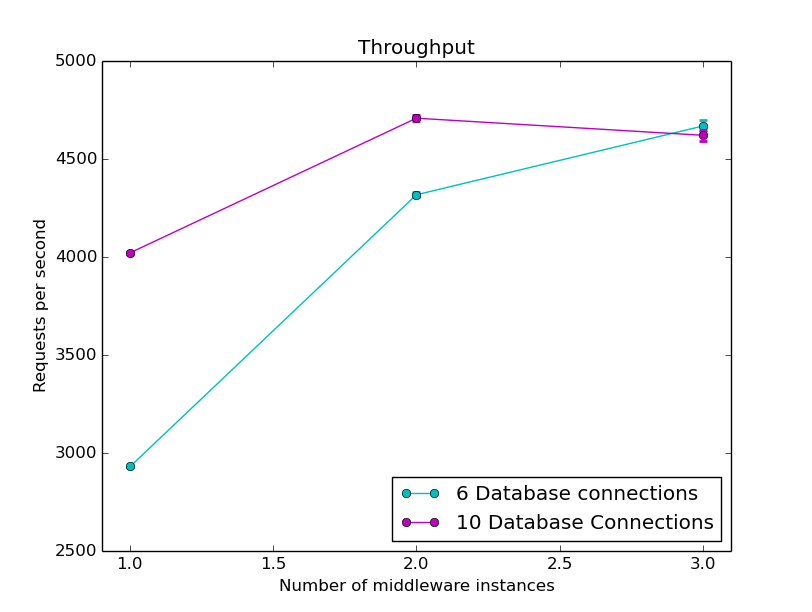
\includegraphics[width=0.7\textwidth,page=1]{figures/scalability_throughput}
  \centering
  \caption{Throughput of the system for different number of middlewares and database
  connections}
  \label{fig:scalability_throughput}
\end{figure}

\begin{figure}[ht]
  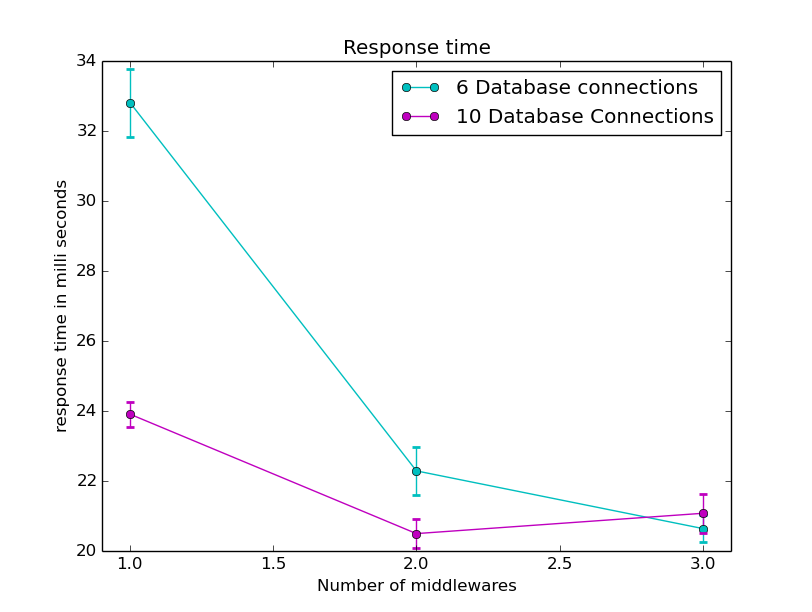
\includegraphics[width=0.7\textwidth,page=1]{figures/scalability_response_time}
  \centering
  \caption{Response time of the system for different number of middlewares and 
  database connections}
  \label{fig:scalability_response_time}
\end{figure}

\subsection{Conclusion}\label{sec:conclusion}
In summary, system in general performs well in terms of throughput and response times as shown in the conducted experiments.
In section \ref{sec:performance-characteristics}, it was shown that system has the highest performance for \emph{15-24}
database connections. Furthermore, as shown in section \ref{sec:performance-characteristics-1}, by using 
\emph{java nio} package and \emph{asynchronous I/O}, one single instance of middleware is able to handle above 
18000 requests per second. However, in this design database is the bottleneck, and system performance is limited 
to the database performance. To make the system highly scalable, one could distribute the database
along several machines, also it could be a good idea to have several instances of the 
\emph{ConnectionManager} to handle the incoming requests asynchronously instead of only one \emph{ConnectionManager} which 
could become a bottleneck under high loads.
If desining the system anew, I would go for the same design, as it was proved in the experiments using the 
\emph{java nio} packages clearly pays off. However, to simplify the design one could use only one \emph{thread\_pool}.
I will also consider another table for the users to authenticate them, also this could be helpful to 
have the information of the users in the database because this way, one does not need to send the user informations
along with their requests, this could help to use a little less bandwidth. 

\end{document}
